\documentclass[12pt]{article}
\usepackage{inputenc}
\usepackage[top=1in, bottom=1in, left=1in, right=1in]{geometry}
\usepackage{setspace}
\usepackage{parskip}
\setcounter{secnumdepth}{1}
\pagestyle{plain}
\usepackage{graphicx}
\setlength{\parindent}{0 cm}
\usepackage[compact]{titlesec}  
\usepackage{amssymb}
\usepackage{amsmath}
\usepackage{float}
\usepackage[hidelinks]{hyperref} % for urls in bibliography
\usepackage{pdfpages} % to insert front page as pdf

\newcommand\numberthis{\addtocounter{equation}{1}\tag{\theequation}}
\titlespacing{\section}{0pt}{0pt}{0pt}

% Bibliography Definition
\makeatletter
% \renewcommand\@biblabel[1]{#1} % No brackets for the references
\def\@biblabel#1{}
\renewenvironment{thebibliography}[1]
     {\section*{\refname}%
      \@mkboth{\MakeUppercase\refname}{\MakeUppercase\refname}%
      \list{\@biblabel{\@arabic\c@enumiv}}%
           {\settowidth\labelwidth{\@biblabel{#1}}%
            \leftmargin\labelwidth
            \advance\leftmargin20pt% change 20 pt according to your needs
            \advance\leftmargin\labelsep
            \setlength\itemindent{-20pt}% change using the inverse of the length used before
            \@openbib@code
            \usecounter{enumiv}%
            \let\p@enumiv\@empty
            \renewcommand\theenumiv{\@arabic\c@enumiv}}%
      \sloppy
      \clubpenalty4000
      \@clubpenalty \clubpenalty
      \widowpenalty4000%
      \sfcode`\.\@m}
     {\def\@noitemerr
       {\@latex@warning{Empty `thebibliography' environment}}%
      \endlist}
\renewcommand\newblock{\hskip .11em\@plus.33em\@minus.07em}
\makeatother


\begin{document}
\includepdf{FrontPage_Project1.pdf}
\section*{Introduction}
	
	\emph{The blood cell population model is an excellent example of a discrete dynamical system taken from biology. It helps illustrate ``how mathematical modeling can be used to explain the behavior and possible origins of dynamical disease.''\footnote{William B. Gearheart, ``A Blood Cell Population Model Dynamical Disease, and Chaos,'' Department of Mathematics; California State University, Fullerton, n.d. Web. 12 Mar. 2014. <\url{http://users.mat.unimi.it/users/naldi/cell.pdf}>} This project will attempt to illustrate the significance of this model as well as investigate its discrete dynamics in terms of stability and chaos.\footnote{Lynch, Stephen, ``Analysis of a Blood Cell Population Model,'' International Journal of Bifurcation and Chaos 15, no. 7 (2005), 2311.}} \footnote{Note: we have been asked to specify the work distribution for this project. Katrina contributed the background research, research on the applications of this model, the powerpoint presentation, the relevant section write-up and helped with compiling the report. Chris focused on the iterative numerics and trajectories, the bifurcation diagrams and wrote up the relevant sections. Gabe contributed the stability analysis of the fixed points, assisted in researching applications and historical significance, wrote up the relevant sections and compiled the final report.}

	On average, the human body contains 5 liters of blood consisting of red blood cells, white blood cells, and platelets. There also exist several types of red and white blood cells. This presents an issue from a mathematical modeling perspective because the ``cellular and biochemical processes involved in [the cells’] dynamics vary considerably.''\footnote{Lynch, 2311.} Regardless of the challenges it presents, studying blood is extremely beneficial because it can be used to diagnose certain diseases in the human population such as ``anemia, chronic renal failure, acute hemorrhaging and marrow failure.''\footnote{Lynch, 2312.}
	
	Red blood cells, or erythrocytes, tend to fluctuate in a healthy human body: woman having 4.2-5.4 per $\mu$L and men 4.7-6.1 per $\mu$L.\footnote{Steven H. Strogatz, ``12.2: The Henon Map.'' In \emph{Nonlinear Dynamics and Chaos: With Applications to Physics, Biology, Chemistry, and Engineering}, Reading, MA: Addison-Wesley Pub., 1994, 50.} It is known that blood cell counts ``can oscillate and even display chaotic behavior'' which is not unexpected, for ``all kids of nonlinear phenomena abound in the human body.''\footnote{Lynch, 2311.} Through application of a blood cell model, these red blood cells can be counted to measure hematologic conditions such as anemia.\footnote{Anemia is a condition marked by a deficiency of red blood cells or of hemoglobin in the blood, resulting in pallor and weariness (\url{www.nhblbi.nih.gov}). It is also defined as, ``Any condition resulting in a significant decrease in total body erythrocyte mass'' (Lynch, p. 285).}\footnote{Strogatz, 59.} It is also helpful to point out that most blood cells are produced by ``primitive stem cells in bone marrow.''\footnote{Lynch, 2312.} The cells are then destroyed through processes such as natural aging, infection, or disease. This cyclic process is represented in the model as a nonlinear phenomenon. 
	
\section*{A Blood Cell Population Model}
	
	A simple blood cell population model was first developed by Polish mathematician, Andrzej Lasota, in 1977.\footnote{Strogatz, 59.} The model he considered was this:
	
	\begin{align}
		c_{n+1} = c_{n} - d_{n} + p_{n}
	\end{align}

	where $c_{n}$ denotes the red cell count at time \emph{n}, and $d_{n}$ and $p_{n}$ represent the number of cells destroyed and produced in the interval, respectively. Furthermore, it is assumed that a constant fraction of cells is destroyed on each iteration, thus $d_{n} = ac_{n}$ where $0 < a \le 1$, and a represents the ``destruction coefficient.''  Also, consider the equation used by Lasota: 
	
	\begin{align}
		p_{n} = bc_{n}^{r}e^{-sc_{n}}
	\end{align}

	where b, c, r, and s are positive constants. Together, these functions give us the blood cell iterative equation used in this project\footnote{Lynch, 2312.}:

	\begin{align*}
		c_{n+1} &= (1-a)c_{n} + bc_{n}^{r}e^{-sc_{n}} \text{ where } \\
		0 &<  a \le 1 \text{ and } b, r, s > 0.
	\end{align*}

	The typical parameters used in the model are $b = 1.1 x 10^{6}$, $r = 8$, and $s = 16$. The analysis of this model is presented in the following sections of this project. Fixed points of period one and the stability of these points will be examined. To supplement the linear stability analysis, bifurcation diagrams will also be plotted as parameters change.\footnote{Lynch, 2314.} This will be implemented through MATLAB.

\section*{Brief Summary}
	Blood Cell Modeling can be utilized in order to explain the behavior and possible origins of dynamical diseases in the human population, such as anemia. A stability analysis can be carried out for a simple blood cell population model, as this project will attempt to demonstrate. Furthermore, bifurcation diagrams can be used to ``establish how the model’s dynamics evolve as parameters vary.'' Please refer to the following sections. 

\pagebreak{}

Consider the blood cell iterative equation $c_{n+1} = (1-a)c_{n}+bc_{n}^{r}e^{-sc_{n}}$.

\section*{Iterative Numerics}
\textbf{Question 1:} Run iterative numerics and describe different types of trajectories.

\textbf{Answer:} 
\begin{figure}[H]
	\begin{center}
    \includegraphics[width=0.8\textwidth]{IterativeNumerics}
    \end{center}
    \caption{Map with 20 different initial conditions, with a = 0.2.}
    \label{Fig. 1}
\end{figure}
Figure 1 plots the map for 20 different initial conditions using typical parameters as described by Lasota in 1977, namely: $b=1.1*10^{-6}, \quad r=8, \quad s=16$. Other possible parameter regimes have also been discussed by Steven Lynch. In general, $a \in [0,1]$, but the `$a$' parameter was chosen in this case to be in a region where the system can converge to one of two stable fixed points depending on the initial conditions. 

\begin{figure}[H]
	\center{center}
    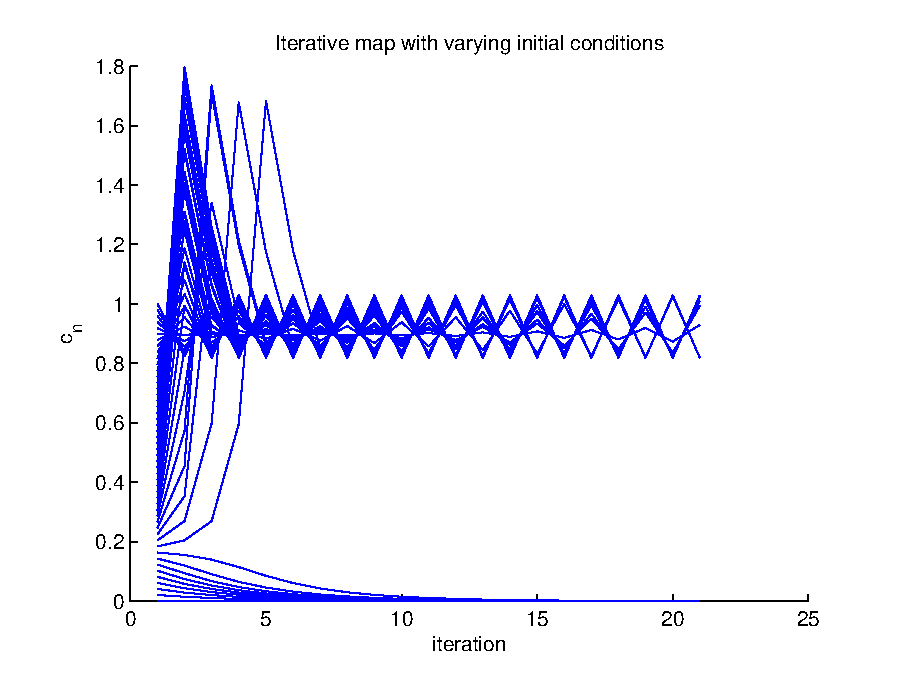
\includegraphics[width=0.8\textwidth]{IterativeNumericsa03}
    \center{center}
    \caption{Map with 20 different initial conditions with parameter a being changed to 0.3.}
    \label{Fig. 2}
\end{figure}
The only change made from figure 1 to figure 2 was the parameter `$a$'. It now lies in a region with one stable solution and a 2-periodic solution. Figure 3 captures all of the behaviours that the system exhibits upon varying '$a$' and the initial condition. At the bottom of the bifurcation diagram we can see that a single stable solution that goes to 0. As '$a$' increases we see orbits of periods 2, 4, and 8 emerge. Then, undoubling of orbits occurs until $a\approx.7$ at which point we see bistability takes place. Figure 4 zooms in on the bistable region. Period doubling begins again at $a\approx .715$ before the system then goes to chaos, but sporadic instances of high periodicity orbits occur for $a \in (.725, .84)$. Figure 5 shows the system eventually becoming a single stable solution at $c_n=0$ for large enough '$a$' and any initial condition. 

\begin{figure}[H]
    \begin{center}
    \includegraphics[width=0.8\textwidth]{Varyac0}
    \end{center}
    \caption{Behaviors of the system exhibited by varying initial conditions.}
    \label{Fig. 3}
\end{figure}
\begin{figure}[H]
	\begin{center}
    \includegraphics[width=0.8\textwidth]{BistableRegion}
    \end{center}
    \caption{Bistable Region}
    \label{Fig. 4}
\end{figure}
\begin{figure}[H]
    \begin{center}
    \includegraphics[width=0.8\textwidth]{chaostoStable}
    \end{center}
    \caption{Chaotic to Stable Behavior}
    \label{Fig. 5}
\end{figure}

\section*{Blood Cell Fixed Point Calculations}
Consider the blood cell iterative equation $c_{n+1} = (1-a)c_{n}+bc_{n}^{r}e^{-sc_{n}}$.

\textbf{Question 2:} Assuming that $b=1.1*10^{6}$, $r=8$ and $s=16$ show that there are two stable and one unstable fixed points of period one when $a=0.2$.

\textbf{Answer:} This question involves both a) finding the fixed points and b) determining the stability of these fixed points. 

Finding Fixed Points: Because we are solving for \emph{period one}, we can solve (a) by finding the intersection points of the line $y=x$ with $f(x) = (1-a)x+(1.1*10^{6})x^{8}e^{-16x}$. Usually we can determine these intersection points using numerical algorithms such as Newton's Method or the Secant Method. In this case, however, we found it difficult to get these methods to converge, so we used graphical estimates. 

If we needed to approximate these roots numerically, we would take a Taylor Expansion of the function and use this in Newton's Method. In our case, however, graphical estimation with MATLAB's `data cursor' yielded fixed points that fulfilled the requirements of the derivative test --- that is, at these fixed points the absolute value of the derivative was greater than or less than 1 with the expected results.

Using the following MATLAB script, the functions and their derivatives were defined symbolically with the `symfun' function and plotted against $y=x$:

\begin{quote}
	\begin{verbatim}
% Set Parameters
a = .2; b = 1.1*10^6; r = 8; s = 16;
% Define Functions and Derivatives
syms x
f = symfun((1-a)*x+b*x^(r)*exp(-s*x),[x]); derivf = diff(f);
a = .3; g = symfun((1-a)*x+b*x^(r)*exp(-s*x),[x]); derivg = diff(g);
y = symfun(x,[x]);
% Plot F(x) vs Y(x)
h1 = ezplot(f,[-.01,1]); hold on; h2 = ezplot(y,[-.01,1]); 
set(h1,`color',`r',`linestyle',`--');
% Set Legend 
legend(`f(x)',`y = x'); xlabel(`x'); ylabel(`f(x) and y(x)');
title(`f(x) = (1-a)*x+b*x^(r)*exp(-s*x) against y(x) = x')
hold off
% Plot G(x) vs Y(x)
h3 = ezplot(g,[-.01,1]); hold on; h4 = ezplot(y,[-.01,1]);
set(h3,`color',`r',`linestyle',`--')
% Set Legend
legend(`g(x)',`y = x');; xlabel(`x'); ylabel(`g(x) and y(x)'); 
title(`g(x) = (1-a)*x+b*x^(r)*exp(-s*x) against y(x) = x')
\end{verbatim}
\end{quote}


With $a=0.2$, this yielded the follow figure which shows that there are at least three fixed points of period one, represented by each intersection: 


\begin{figure}[H]
    \begin{center}
    \includegraphics[width=\textwidth]{P1_Q2}
    \end{center}
    \caption{Here we can see that there are at least three fixed points of period one as there are three intersections. Note: the graph has cut off the top of the function for the sake of seeing the intersection points. The behavior of the function is simply concave and reprsents something close to a parabola in this window. For a further picture, see the attached graph at the end of this section.}
    \label{figure:2.1}
\end{figure}

Using MATLAB's `data cursor' we can identify these points as $x\text{*}_{1} = 0$, $x\text{*}_{2} = 0.16$ and $x\text{*}_{3} = 0.94$. The next step in our analysis is to find the stability at these points.

Determining Stability: Stability at these fixed points is determined by calculating the absolute value of the derivative at the fixed points. If this value is less than 1, then the fixed point is stable; if it is greater than 1, then the fixed point is unstable. In other words,

\begin{align*}
abs(f'(x\text{*})) &< 1 \rightarrow \text{fixed point is stable} \\
abs(f'(x\text{*})) &> 1 \rightarrow \text{fixed point is unstable}
\end{align*}

For this system in general, we find that the derivative is:

\begin{align*}
	\frac{df}{dx\text{*}}((1-a)x\text{*} + bx\text{*}^{r}e^{-sx\text{*}}) &= (1-a) + (r)bx\text{*}^{r-1}e^{-sx\text{*}} + (-s)bx\text{*}^{r}e^{-sx\text{*}} \\
	&= (1-a) + bx\text{*}^{r-1}e^{-sx\text{*}}(r-sx\text{*}) \\	
	&= (1-a) + bx\text{*}^{r}e^{-sx\text{*}}\frac{r-sx\text{*}}{x\text{*}}\\
\end{align*}

Furthermore, with this result, we find that:

\begin{align*} 
	\frac{df}{dx\text{*}} &< 1 \text{ when } a > bx\text{*}^{r-1}e^{-sx\text{*}}(r-sx\text{*})
\end{align*}

We could use this result to determine stability at fixed points for any given set of parameters at any given fixed point. In our case, however, we have used MATLAB's symbolic toolbox to calculate the derivatives, seen as `derivf = diff(f)' in the code above. We can then calculate the absolute value of the derivatives at those points yielding the following results:


\begin{table}[h]
\centering
\begin{tabular}{rrr}
Fixed Point & Abs(f'(x*)) & Stability \\
0           & 0.8000      & stable    \\
0.16        & 2.0418      & unstable  \\
0.94        & 0.6759      & stable   
\end{tabular}
\end{table}

Thus, we have shown that there are two stable fixed points and one unstable fixed point within this system when $a = 0.2$.

\textbf{Question 3:} Assuming that $b=1.1*10^{6}$, $r=8$ and $s=16$ show that there are one stable and two unstable fixed points of period one when $a=0.3$.

\textbf{Answer:} We use the same techniques as the last problem in order to show this to be true.

Here is the graph that is generated by plotting $y=x$ against our $g(x) = (1-a)x+(1.1*10^{6})x^{8}e^{-16x}$ where $a = 0.3$: 

\begin{figure}[H]
    \begin{center}
    \includegraphics[width=\linewidth]{P1_Q3}
    \end{center}
    \caption{Here, again, we can see that there are at least three fixed points of period one as there are three intersections.}
    \label{figure:2.1}
\end{figure}

Upon analysis with MATLAB's `data cursor', it was found that the fixed points seem to differ slightly with values of $x\text{*}_{1} = 0$, $x\text{*}_{2} = 0.17$ and $x\text{*}_{3} = 0.89$. Taking the derivatives at these points yields the expected results of two unstable fixed points and one stable fixed point: 

\begin{table}[h]
\centering
\begin{tabular}{rrr}
Fixed Point & Abs(g'(x*)) & Stability \\
0           & 0.7000      & stable    \\
0.17        & 2.2700      & unstable  \\
0.89        & 1.2859      & unstable   
\end{tabular}
\end{table}

\section*{Complete Diagram of Function from $x = -0.1 \text{ to } 1$}
\begin{figure}[H]
    \begin{center}
    \includegraphics[width=\linewidth]{P1_CompleteGraph}
    \end{center}
    \caption{Here we see the complete graph of the function, particularly the parabolic aspect which was cut off in the previous pictures. Furthermore, our function appears to lie underneath the diagonal as Cn approaches infinity. This suggests that these may be the only fixed points for this system of period one, although there are fixed points of other periods.}
    \label{figure:2.1}
\end{figure}


% Begin Bibliography
\pagebreak
\begingroup
\renewcommand{\section}[2]{}	% in article, this becomes reference, so we suppress the normal \section\refname
\centerline{\textbf{Bibliography}} 
\begin{thebibliography}{9}
\bibitem{Bifurcation}
\url{Dictionary.com}. ``Bifurcate.'' \emph{Dictionary.com}. \url{http://dictionary.reference.com/browse/bifurcate}. (accessed March 26, 2014)
\bibitem{Bifurcation}
Weisstein, Eric W. ``Bifurcation.'' From MathWorld---A Wolfram Web Resource. \url{http://mathworld.wolfram.com/Bifurcation.html}
\bibitem{Gearhart}
Gearhart, William B. , and Mario Martelli. ``A Blood Cell Population Model, Dynamical Diseases, and Chaos.'' Department of Mathematics; California State University, Fullerton. \url{http://users.mat.unimi.it/users/naldi/cell.pdf} (accessed March 12, 2014).
\bibitem{Lynch_1}
Lynch, Stephen. ``Analysis of a Blood Cell Population Model.'' International Journal of Bifurcation and Chaos 15, no. 7 (2005): 2311-2316.
\bibitem{Lynch_2}
Lynch, Stephen. ``Chapter 12.'' \emph{Dynamical Systems with Applications Using Mathematica}. Boston, MA: Birkh\"{a}user, 2007. N. pag. Print.
\bibitem{Strogatz}
Strogatz, Steven H. ``12.2: The Henon Map.'' In \emph{Nonlinear Dynamics and Chaos: With Applications to Physics, Biology, Chemistry, and Engineering}. Reading, MA: Addison-Wesley Pub., 1994.
\bibitem{Anemia}
``What Is Anemia?.'' - NHLBI, NIH. \url{https://www.nhlbi.nih.gov/health/health-topics/topics/anemia/} (accessed March 22, 2014).
\end{thebibliography}
\endgroup

\pagebreak{} % so we do not overlap with bibliography
\section*{MATLAB Appendix: \\ Scripts for Generating Bifurcation Diagrams and Iterative Numerics}

\begin{verbatim}
function bloodModelVaryac0(steps,b,r,s)

% Pressing "Run" button uses the below values as the inputs
%   for the function.
if(nargin==0)
    steps=200;
    b=1.1*10.^6;
    r=8;
    s=16;
end

ICs=10; % Number of initial conditions
c0=linspace(0,1,ICs); % Initial conditions tested between 0 and 1.5
runs=70; % Number of different `a' values to test
a=linspace(.6,.75,runs).'; % Linearly spaced vector of `a' values
cn=zeros([1, steps]); 

%Starts clock on main loop
t=cputime;

% Loop through initial condition values
for k=1:ICs
    cn(1)=c0(k);    
    % Loop through the `a' values
    for j=1:runs    
        % Loop through the first (steps-50) steps
        for i=1:steps-50
        cn(i+1)=(1-a(j)).*cn(i)+b*cn(i).^r*exp(-s*cn(i));
    end
    
    % Plots new data on the same graph
    hold on
    
    % Loop through final steps while plotting bifurcation diagram.
    % Plotting just these steps ensures that we only use values that 
    %   are in the periodic orbits that the map converges to for a given
    %   `a'.
    for i=steps-50:steps
        cn(i+1)=(1-a(j)).*cn(i)+b*cn(i).^r*exp(-s*cn(i));
        plot(a(j), cn(i),`-', `MarkerSize',2);
    end
    end
end
% Determines how long the main loop takes to run
loopTime=cputime-t;
display(loopTime);

xlabel(` a ');
ylabel(` c_n for last 50 values')
title(`Bifurcation diagram found by varying ``a''');

end

---

function bloodModelr5(c0,steps,b,r,s)

% Pressing ``Run'' button uses the below values as the inputs
%   for the function.
if(nargin==0)
    c0=1; % Initial condition
    steps=100; % Number of iterations of the map
    b=1.1*10.^6; % Value of parameter given in part (b)
    r=4.9;         % "                                  "
    s=16;        % "                                  "
end

a=.2; % Value given in part (b)
% a=.3;  % Value given in part (c) 
cn=zeros([1,steps]); % Create a vector to hold value at each step
cn(1)=c0; % Initial condition
    
% Main loop to generate iterative map
for i=1:steps
    cn(i+1)=(1-a).*cn(i)+b*cn(i).^r*exp(-s*cn(i));
end

% Simple plot of result
figure
plot(cn(:));
end

---
function bloodModelSimple(c0,steps)

if(nargin==0)
    c0=linspace(0,1,50);
    steps=20;
end
a=.3;
b=1.1*10.^6;
s=16;
r=8;
cn=zeros([1 steps]);
xlabel(`iteration');
ylabel(`c_n');
title(`Iterative map with varying initial conditions');
for k=1:50
    cn(1)=c0(k);
    for j=1:steps
        cn(j+1)=(1-a).*cn(j)+b*cn(j).^r*exp(-s*cn(j));
    end
    hold on
    plot(cn,`-');
end
end

---
function bloodModelSinglea(c0,steps,b,r,s)

if(nargin==0)
    c0=1.5;
    steps=1000;
    b=1.1*10.^6;
    r=8;
    s=16;
end

runs=200;
a=linspace(0,1,runs).';
cn=zeros([1, steps]);
cn(1)=c0;

for j=1:runs
    
    for i=1:steps-100
        cn(i+1)=(1-a(j)).*cn(i)+b*cn(i).^r*exp(-s*cn(i));
    end
    hold on
    for i=steps-100:steps
        plot(a(j), cn(i),`-', `MarkerSize',2);
    end
end
end


---

function bloodModelVaryA(c0,steps,b,r,s)

% Pressing "Run" button uses the below values as the inputs
%   for the function.
if(nargin==0)
    c0=1.5;
    steps=300;
    b=1.1*10.^6;
    r=8;
    s=16;
end

runs=500; % Number of different `a' values to test
a=linspace(0,1,runs).'; % Linearly spaced vector of `a' values
cn=zeros([1, steps]); 
cn(1)=c0;

% Loop through the `a' values
for j=1:runs
    
    % Loop through the first (steps-50) steps
    for i=1:steps-50
        cn(i+1)=(1-a(j)).*cn(i)+b*cn(i).^r*exp(-s*cn(i));
    end
    
    % Plots new data on the same graph
    hold on
    
    % Loop through final steps while plotting bifurcation diagram.
    % Plotting just these steps ensures that we only use values that 
    %   are in the periodic orbits that the map converges to for a given
    %   `a'.
    for i=steps-50:steps
        cn(i+1)=(1-a(j)).*cn(i)+b*cn(i).^r*exp(-s*cn(i));
        plot(a(j), cn(i),`-', `MarkerSize',2);
    end
end

xlabel(` a ');
ylabel(` c_n for last 100 n values')
title(`Bifurcation diagram found by varying "a"');

end


---

function bloodModelVaryac0(steps,b,r,s)

% Pressing "Run" button uses the below values as the inputs
%   for the function.
if(nargin==0)
    steps=200;
    b=1.1*10.^6;
    r=8;
    s=16;
end

ICs=10; % Number of initial conditions
c0=linspace(0,1,ICs); % Initial conditions tested between 0 and 1.5
runs=70; % Number of different `a' values to test
a=linspace(0,1,runs).'; % Linearly spaced vector of `a' values
cn=zeros([1, steps]); 

%Starts clock on main loop
t=cputime;

% Loop through initial condition values
for k=1:ICs
    cn(1)=c0(k);    
    % Loop through the `a' values
    for j=1:runs    
        % Loop through the first (steps-50) steps
        for i=1:steps-50
        cn(i+1)=(1-a(j)).*cn(i)+b*cn(i).^r*exp(-s*cn(i));
    end
    
    % Plots new data on the same graph
    hold on
    
    % Loop through final steps while plotting bifurcation diagram.
    % Plotting just these steps ensures that we only use values that 
    %   are in the periodic orbits that the map converges to for a given
    %   `a'.
    for i=steps-50:steps
        cn(i+1)=(1-a(j)).*cn(i)+b*cn(i).^r*exp(-s*cn(i));
        plot(a(j), cn(i),`-', `MarkerSize',2);
    end
    end
end
% Determines how long the main loop takes to run
loopTime=cputime-t;
display(loopTime);

xlabel(` a ');
ylabel(` c_n for last 50 values')
title(`Bifurcation diagram found by varying ``a''');

end

---

function bloodModelvaryr(c0,steps,b,s)

% Pressing "Run" button uses the below values as the inputs
%   for the function.
if(nargin==0)
    c0=.5; % Initial condition
    steps=300; % Number of iterations of the map
    b=1.1*10.^6; % Value of parameter given in part (b)
    s=16;        % "                                  "
end

rVals=300;
r=linspace(0,10,rVals);
% a=.2; % Value given in part (b)
a=.3;  % Value given in part (c) 
cn=zeros([1,steps]); % Create a vector to hold value at each step
cn(1)=c0; % Initial condition

t=cputime;
% Main loop to generate iterative map
for k=1:rVals
    
    for i=1:steps-100
        cn(i+1)=(1-a).*cn(i)+b*cn(i).^r(k)*exp(-s*cn(i));
    end
    hold on
    for i=steps-100:steps
        cn(i+1)=(1-a).*cn(i)+b*cn(i).^r(k)*exp(-s*cn(i));
        plot(r(k),cn(i),`-', `MarkerSize',2);
    end
end
loopTime=cputime-t;
display(loopTime);
xlabel(` r ');
ylabel(` c_n for last 50 values')
title(`Bifurcation diagram found by varying "r"');
end

---

function bloodModelVarys(c0,steps,b,r)

% Pressing "Run" button uses the below values as the inputs
%   for the function.
if(nargin==0)
    c0=.5; % Initial condition
    steps=200; % Number of iterations of the map
    
    b=1.1*10.^6; % Value of parameter given in part (b)
    r= 8;        % "                                  "
    % s=16;        % "                                  "
end

sVals=200;
s=linspace(8,20,sVals);
% a=.2; % Value given in part (b)
a=.3;  % Value given in part (c) 
cn=zeros([1,steps]); % Create a vector to hold value at each step
cn(1)=c0; % Initial condition

t=cputime;
% Main loop to generate iterative map
for k=1:sVals
    
    for i=1:steps-20
        cn(i+1)=(1-a).*cn(i)+b*cn(i).^r*exp(-s(k)*cn(i));
    end
    hold on
    for i=steps-20:steps
        cn(i+1)=(1-a).*cn(i)+b*cn(i).^r*exp(-s(k)*cn(i));
        plot(s(k),cn(i),`-', `MarkerSize',2);
    end
end
loopTime=cputime-t;
display(loopTime);
xlabel(` r ');
ylabel(` c_n for last 20 values')
title(`Bifurcation diagram found by varying "s"');
end

---

function c0findBifurcation
    format long
    upper=.2;
    lower=.1;
    steps=50;
    a=.3;
    b=1.1*10.^6;
    s=16;
    r=8;
    cn=zeros([1 steps]);
    c0=.15;
    tol = 1*10.^(-13);
    c0temp=1;
    while abs(c0temp-c0) > tol
        
        cn(1)=c0;
        for j=1:steps-1
            cn(j+1)=(1-a).*cn(j)+b*cn(j).^r*exp(-s*cn(j));
        end
        if cn(steps)< .5
            c0temp=c0;
            lower=c0;
            c0=(upper+c0)/2;
        else
            c0temp=c0;
            upper=c0;
            c0=(lower+c0)/2;
        end
    end
    display(c0);

\end{verbatim}


\end{document}

